% Name: Empirical distribution function
% Description: The step function of ten observations, rising by one tenth at each value, with closed dots where each step starts and open dots where it ends.
% Tags: step function, empirical CDF, statistics, distribution

\usepackage{pgfplots}
\pgfplotsset{compat=1.18}

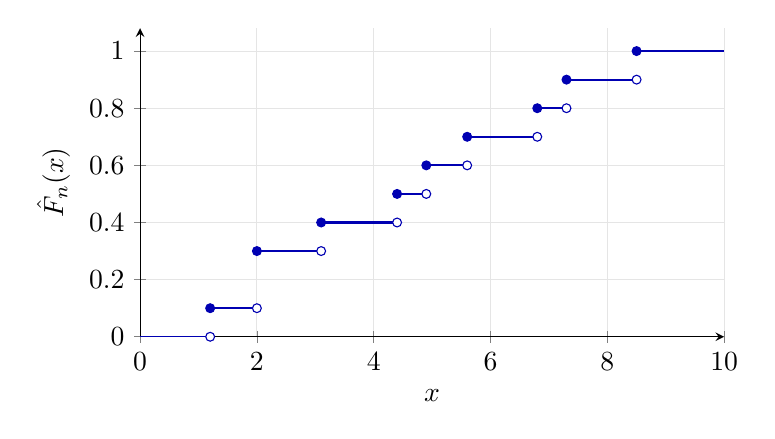
\begin{tikzpicture}
  \begin{axis}[
    width=9cm, height=5.5cm, xmin=0, xmax=10, ymin=0, ymax=1.08,
    xlabel=$x$, ylabel={$\hat F_n(x)$}, ytick={0,0.2,...,1},
    grid=major, grid style={gray!20}, axis lines=left,
  ]
    % Observations: 1.2, 2.0, 2.0, 3.1, 4.4, 4.9, 5.6, 6.8, 7.3, and 8.5; the value 2.0 appears twice, so its step is 0.2.
    \addplot[blue!70!black, thick, jump mark left] coordinates {
      (0,0) (1.2,0.1) (2.0,0.3) (3.1,0.4) (4.4,0.5) (4.9,0.6) (5.6,0.7) (6.8,0.8) (7.3,0.9) (8.5,1) (10,1)
    };
    \addplot[only marks, mark=*, mark size=1.6pt, blue!70!black] coordinates {
      (1.2,0.1) (2.0,0.3) (3.1,0.4) (4.4,0.5) (4.9,0.6) (5.6,0.7) (6.8,0.8) (7.3,0.9) (8.5,1)
    };
    \addplot[only marks, mark=*, mark size=1.6pt, mark options={fill=white, draw=blue!70!black}] coordinates {
      (1.2,0) (2.0,0.1) (3.1,0.3) (4.4,0.4) (4.9,0.5) (5.6,0.6) (6.8,0.7) (7.3,0.8) (8.5,0.9)
    };
  \end{axis}
\end{tikzpicture}
